\section{MapReduce}
\subsection{Présentation et fonctionnement}

\par MapReduce est un patron d'architecture de développement informatique, inventé par Google. Un de ses principaux objectifs est de réaliser des calculs parallèles et souvent distribués sur des jeux de données très volumineuses (de l'ordre du téraoctet, voire du pétaoctet).

\par Un programme MapReduce met généralement en o\oe{}vre à la fois des tâches de type \textit{map} et \textit{reduce}. L'adoption de ce patron est liée au fait qu'un développeur Hadoop peut ne plus se soucier de l'ensemble des enregistrements mais peut raisonner uniquement sur un seul enregistrement lors de l'écrire de l'algorithme. Ainsi, le passage d'un enregistrement à un autre ainsi que la détection de la fin du fichier sont pris en compte par Hadoop.

\par Le fonctionnement de MapReduce se décompose en trois parties :
\begin{itemize}
\item le \textit{driver} s'exécutant sur une machine et chargé de configurer le job et de le soumettre pour exécution (cf \ref{sec:matmult});
\item le \texttt{mapper} chargé de lire les données dans le HDFS et de les traiter;
\item le \texttt{reducer} chargé de consolider les résultats issus du \texttt{mapper}, de les écrire sur le HDFS. L'utilisateur peut ensuite les récupérer sur son disque local.
\end{itemize}

\begin{figure}[h!]
  \centering
  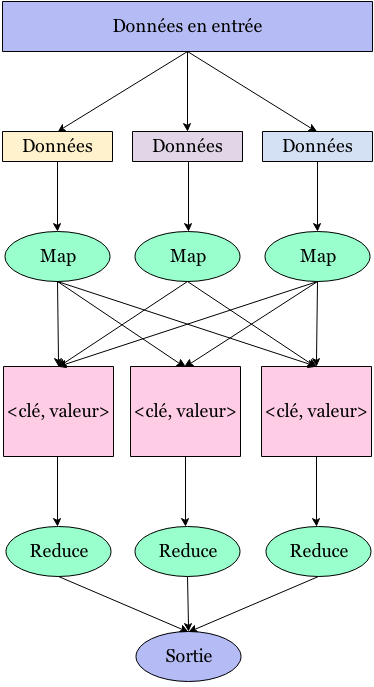
\includegraphics[scale=0.4]{images/mapreduce_arch.png}
  \caption{Architecture du patron MapReduce}
  \label{fig:mapreduce-exp}
\end{figure}

\par La figure~\ref{fig:mapreduce-exp} donne l'aperçu global du patron MapReduce. Les données présentées en entrée sont splittées. Concrètement, les données splittées correspondent tout simplement aux blocs stockés dans les DataNodes des fichiers (cf \ref{sec:hdfs}). C'est sur ces données que va s'exécuter la fonction \textit{map} dans un premier lieu. La particularité c'est que c'est le code qui est envoyé sur les noeuds esclaves et non les données qui y sont déjà présentes. En terme d'I/O, les performances de calculs sont considérablement augmentées puisqu'on s'épargne le temps de transfert des données.

\par Plusieurs fonctions \textit{map} peuvent s'exécuter simultanément. Ceci est possible du fait de l'architecture maître-esclave. La parallélisation des calculs augmente donc le temps de traitement.

\subsection{Les I/O}
\label{sec:mapreduce-io}

\par Dans un algorithme MapReduce, les données présentes en entrée/sortie des tâches \textit{map} et \textit{reduce} sont toujours sous la forme \texttt{<key, value>} ou \texttt{<clé, valeur>}. Imposer cette structure unique et simple aux enregistrements contribue à l'efficacité d'Hadoop au niveau des I/O.

\subsection{La fonction \textit{map}}

\par Le programme le plus simple permettant de comprendre le patron MapReduce est le \texttt{wordcount}. Celui-ci permet de compter le nombre d'occurrences des mots d'un ou plusieurs fichiers. Afin d'illustrer la fonction nous prenons cet exemple. Le code source Java ainsi que les \texttt{input} et \texttt{output} sont joints à ce rapport.

\paragraph{Le << parsage >> des données.} Un fichier texte en entrée de la fonction \textit{map} est traitée de façon très spécifique. En effet, la fonction \textit{map} prend en entrée une ligne du fichier. Le fichier ci-dessous

\begin{quote}
banane wiki mangue mac toto\\
mac kiwi galaxy banane kiwi\\
\end{quote}

présenté en entrée de la fonction \textit{map} du \texttt{wordcount} produira le jeu de <clé, valeur> suivant :\\

\centerline{
\begin{tabular}{|c|c|}
\hline  1ère phrase & 2ème phrase \\ 
\hline banane, 1 & mac, 1\\wiki, 1 & kiwi, 1\\ mangue, 1 & galaxy, 1\\ mac, 1 & banane, 1\\ toto, 1 & kiwi, 1\\
\hline 
\end{tabular}} 

\subsection{La fonction \textit{reduce}}



%%% Local Variables: 
%%% mode: latex
%%% TeX-master: "CompteRendu"
%%% End: 